\documentclass{article}

\usepackage{a4}
\usepackage{graphicx}

\begin{document}

\title{The Engine Behind Model Checking}

\maketitle

\begin{abstract}
In order to ensure the safety and quality of a system, it is necessary to undergo a process of system validation which checks the correctness of specifications, designs and products. The various validation techniques are peer reviewing, simulation, formal verification, and model checking, etc. Of all the techniques, model checking has become the most popular approach in the both hardware and software areas due to the availability of various support tools and its success in the project. This report gives a brief introduction about the fundamentals of model checking. Various terminologies used related to model checking is also described. It also provides the fundamental approaches to model checking along with their examples. It will also introduce some of the model checkers. SAT-Technology is emerging as a central engine used in model checking tools. The principle behind it is very simple: formulate everything at the (logical) gate-level, and then run a SAT solver. The devil is then in the details. This project is about exploring this fascinating and recent connection. Either gaining some overview, or exploring a concrete application. The model, the logical side of it, the SAT side of it is a planned task for the initial document to write.

\end{abstract}

\tableofcontents



\section{Introduction}
\label{sec:intro}

Describing what a system is required to do is known as system specification. By doing so, we will be able to understand the system. Various validation techniques are used to check the correctness of specification. It guarantees the quality of the system and also its safety [6]. Model checking is one of the most popular validation techniques. For a system defined in finite state model and a property defined in terms of logical formalism, model checking techniques could systematically check the validity of this property [10]. A finite-state model is used to design computer programs and digital logic circuits. It is as an abstract machine that can be in one of a finite number of states. It will be only in one state at a time; the state it is in at any given time is called the current state. When initiated by a triggering event or condition, the state changes, this is called a transition.
Roughly, M is an abstract model of a system whose structure is defined as finite-automata and $\Phi$ is a logical formula specifying a desirable property such that M satisfies $\Phi$ abbreviated as $M \models \Phi$.
Model checking helps from preventing the bugs even before penning down the code of the project i.e., during the requirement and the design phase itself. It prevents the further breed of the bugs and hence it makes sense by being cost effective [5]. The errors which are not been able to find by simulation is done by model checking by considering all possible behaviours of the system [2].


\subsection{Systems and their Specifications}
\label{sec:SystemsSpec}

Describing a system is called specification. Specification helps in finding errors and    understanding a system. So, it is a good practise to have a clear idea about the design and improve it before the implementation. The specification of the system can be functional or non-functional i.e. what a system is supposed to do or performance properties. These specifications are written in formal language with proper syntax and semantics which can be verified and validated with respect to requirements.
It helps in developing the explicit model of a system which is clear, precise and unambiguous. Mathematics is used as a basic tool to achieve this. Here, reading the accompanying words in order to understand the relation between the equations is a bit tedious. In order to overcome this shortcoming using mathematics as a basic tool, logicians have temporal logic which is precise and completely formal mathematics. This temporal logic is used in such a way so as to describe the system behaviour.


\subsection{Temporal Logic}
\label{sec:templog}

There are various interpretations of temporal logic depends on the individual as how to consider the system with time. It is the logic for expressing mathematics. It supports formulating the properties of the system behaviour with respect to time. There are various types of temporal logics:
\begin{enumerate}
\item Temporal Logics used to specify the reactive systems are:
  \begin{enumerate}
  \item Linear temporal logic:  It allows the statement of properties of execution sequences of a system.
  \item Branching temporal logic: It allows the user to write formulas which include some sensitivity to the choices available to a system during its execution.
  \end{enumerate}
These two kinds o`f temporal logic are characterized by a continuous interaction with the environment [10].
\item Temporal Logics used to specify the time-critical systems:

Real-Time temporal logic: It allows statement of properties of multiple concurrent processes and supports relative time references.
\end{enumerate}

It is characterized by quantitative timing properties relating occurrences of events [10].
In order to avoid the errors we write specifications. Validation techniques are used to checking the correctness of the system.



\section{Model Checking}
\label{sec:modelchecking}

The technique used for validating a system is Model checking. The design process and the validation process are the must to ensure the correctness of specifications, designs and products of the system. Validation is done to see that whether the system meets all its requirements.
The two types of validation techniques are:
\begin{itemize}
\item[\textbf{.}]Informal ones which include peer testing and testing.

\end{itemize}	
\begin{itemize}
\item[\textbf{.}]Formal ones which include formal verification, simulation and model checking.

\end{itemize}	
This report focuses on the Formal validation technique – Model Checking.
Model checking systematically checks the validity of a given finite-state model of a system and properties stated in the form of logical formalism such as temporal logic. It uses algorithms which are executed by the computer tools. The inputs to such model checkers are the description of the model and the description of the properties. Once these files are fed as an input, the model checker performs the verification. If error occurs, then the model checker provides the counter-example to explain under which circumstances the error can be generated. This counter-example helps in finding the error and repairing the specifications of the model. This can be shown with help of the following diagram. It shows us how the verification process takes place in the model checking.

\subsection{Specified Property}
\label{sec:specprop}

\begin{description}
\item[Liveness] The properties, at any particular instance, which can’t be violated.
\item[Fairness] If this step is enabled continuously then property asserts the step eventually.
\item[Safeness] The system requirements which do nothing.
\item[Deadlock] It checks if the system is freed from dead locks.
\item[State properties] It checks if the model has some state.
\item[Time requirement] The property specifying time requirements of the system.
\end{description}


\subsection{Model Checking Algorithm}
\label{sec:modcheckalg}

Model checking uses exhaustive state space search of the system model as 	algorithm: The desired properties satisfied for each state of the model. 	Reachability property is used to check whether the system can reach a state without any deadlocks. Reachability is considered as one of the important property which uses Reachability analysis technique. It starts from initial system state and see to it that it reaches all the possible system states which can be reached. For instance, in a traffic signal model, yellow, red and green are the three states. Model checking proves if it can reach some state, all the states are eventually got by the model, or if the model could never get some state.


\subsection{Approaches of Model Checking}
\label{sec:approchmodcheck}

\begin{itemize}
\item[\textbf{.}] Logic based approach: Here the system is modelled as finite-state automaton representing the states as values of variables and control location, and changes of a system from one state to other state is represented by transition. If a system satisfying the desired behaviour given in some logic with the initial set of states, then the system is said to be correct.

\end{itemize}
\begin{itemize}
\item[\textbf{.}]	Behaviour based approach: Given the desired and the possible behaviour with the same notation, the equivalence relations are used as criteria for the correctness. Hence, if the desired and the possible state behaviour are equivalent then the system is said to be correct.
\end{itemize}



\section{Model Checkers}
\label{sec:modelcheckers}

In verifying a system, model checking techniques uses tools known as model checkers. Due to the progress of model checking, industries are developing their own model checkers.
Few of the lists of tools are:
\begin{enumerate}
\item  Blast model checker: Berkeley Lazy Abstraction Software Verification Tool abbreviated as BLAST. It is a model checking tool used for C programs.
\item Java path finder: The executable java byte code programs are verified by this java pathfinder system. It does the model checking for the concurrent programs .As using this it helps in detecting the deadlocks and data races. It can also be used to model check the distributed applications and user interfaces.
\item Moon Walker: It model checks for .Net applications by detecting the errors. Also it is able to find the deadlocks and assertion violations as well.
\item Spin Model Checker: It verifies the correctness of the models in automated fashion. This is one of the biggest achievements. It avoids preconstruction of the states.
item UPPAAL: It is used for real-time systems for modelling, validation and verification.
\item TLA+: It is commonly called as Temporal Logic of Actions. It combines logic of actions with temporal logic. In concurrent systems TLA+ is used in describing its behaviour.
\end{enumerate}



\section{Technology}
\label{sec:Technology}

Model checking then, used explicit state traversal where the reachable state space was traversed to find the errors violating the safety properties. It consumed lot of space in the computer memory because each state of the system was stored in large hash table. In order to improve this space consumption in explicit state model checker various techniques came into existence. SPIN model checker was the most successful explicit model checker. The goal of this was to overcome the state explosion problem where the states of the model were represented symbolically.
Later in mid-80’s Binary Decision Diagrams as a new data structure came into existence for symbolical representation and manipulating Boolean functions efficiently [4] known as Symbolic model checking with BDDs. BDDs could handle much larger designs with hundreds of state variables representing Boolean functions. There existed some shortcoming in BDDs as well. They became too large to handle as they used canonical representation. BDDs required uniform variable ordering along the paths and it sometimes happened that no space efficient variable ordering existed. This was time consuming and needed manual intervention.
There came into existence the SAT procedures as an alternative approach to model checking. Unlike BDDs, it didn’t use the canonical representation. It became one of the most efficient implementation. It overcame the state explosion problem faced by BDDs.
In late 90s, researchers came up with the idea of Bounded model checking which uses SAT solvers to the model checking problem. Bounded model checking technique do a fast exploration of state space overcoming the shortcomings of the previous approaches using the SAT procedures instead of BDDs where the SAT has a depth first search nature. This method is applicable for properties which include safety and liveness where it checks whether a given set of states is reachable, and detects loops in a system’s state transition graph.


\subsection{Example to illustrate the new technique}
\label{sec:exampleillust}

Application of Model Checking ranges from simple coffee machines to nuclear plants which are undoubtedly critical and the failure of which may cause economical and physical damages. Considering an example of a coffee machine, where the system is fed with a sensitive data to check the behaviour of the system as it is supposed to behave. This is known as testing.


% \begin{figure}[h!]

%   \centering
%     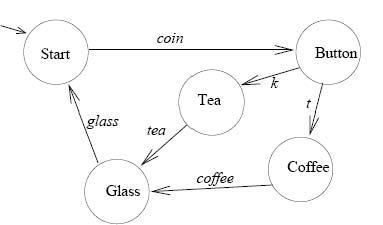
\includegraphics[width=0.5\textwidth]{flower.png}
%     \caption{Finite states of a coffee machine.}
% \end{figure}


A coffee machine consists of a set the following above states which are depicted in circles and relations as arrows between the states. Arrows are given with labels representing actions. The combination of this set of states and relations is known as “automaton”.  If the given action on an arrow connecting both the states is satisfied, then automaton in a given state changes to another state.



Initially the machine is at state "Start" and it "waits" for a coin. If a coin is provided then the machine change state to the "Button" state where two options are possible: to press the "k" button and then go to the "Coffee" state, or to press "t" and go to the "Tea" state. After serving the corresponding drink, the machine goes to the "Glass" state and it gives a glass with the chosen drink to then go back to the "Start" state.


Example 1.
The property "Always, after the machine gets a coin and the user press a button, it gives coffee or tea", can be written in temporal logic as:
ALWAYS (IF Button THEN (SOMETIME-IN-THE-FUTURE (Coffee OR Tea)))
Words in uppercase are temporal logic "connectives" or "operators", and the other words represent the interaction between the machine and the user. The above expression is a "formula" of temporal logic.
How can one see that the given automaton satisfies a formula? We can explain it by using the above formula and the automaton modelling the coffee machine.
Let us assume the current state of the automaton is the initial "Start" state. Let A and B be statements, then "ALWAYS A" means that A must be true in all the states of the automaton. "IF A THEN B" means that whenever A is true in a given state, so is B. "A OR B" means that at least one of A and B must be true in the state. Finally "SOMETIME-IN-THE-FUTURE A" means that it must exist a state in the future of the current state where A is true.
It is then possible to check that the above formula is satisfied by the automaton, since from the state "Button" (after a coin is inserted) it is possible to find a state in the future such that the actions "coffee" or "tea" are possible.



Example 2.
Let us consider now the following property: "Always, after pressing a button the machine will serve coffee and then tea immediately afterwards". We can write this sentence as follows:
ALWAYS (IF Button THEN (Coffee AND NEXT Tea))
Here NEXT is a connective formalising the "immediately after" English expression. As for the previous example it is possible to check whether the automaton satisfies the property. In this case we can see that it is not the case, since from the state "Button" one can reach the state "Coffee" and "Tea", but from the "Coffee" state it is not possible to go immediately after to the "Tea" state. This property guarantees that the machine will never allow to get coffee and then tea by paying only once.



\section{Challenges facing}
\label{sec:challenges}

\begin{enumerate}

\item Learning the usage of Github: It is a website used for storing and presenting our files. Git is a decentralized version control system that is used by a number of open source projects, most notably perhaps the Linux kernel. GitHub is a new hosted Git repository service that's being called a "social network" for programmers and with good reason. In my project it helps in communication between me and my supervisor by providing information to assist in evaluating the tools and making an informed decision.

\item Learning the usage of LATEX: It is a document preparation system similar to that of a Microsoft word where the similarities end here. Preparing a document with LATEX consists of using a text editor to edit a Latex source file with the .tex extension. And then running a latex program to convert the source file to a document interchange format like PDF etc. Doing in LATEX provides a good typography which provides a good impression on the content of the document and is platform independent unlike MS word which runs only on windows. It's much better than copy+paste since it can be changed by changing just the definition. Even more, Latex allows people to write programs in their documents.

\end{enumerate}



\section{Conclusion}

Model checking is used in many areas including both the hardware the software fields. It helps in considering only subset of the system requirements leading to the improved efficiency by supporting partial verifications. Compared to simulation and testing, model checking uses shorter time for verification as shown by many case studies. It can also deal with the states which are larger.


There are shortcomings that still need to be answered:
\begin{itemize}
\item There is no way to translate automatically the requirements into its own modelling language defined by its model checking tool. This has to be done manually.
\item Some of the properties which are to be verified are difficult to express in the notation.
\item Model checking involves much number of states consuming extra efforts in checking parts of the model separately.
\end{itemize}
Despites these shortcomings the model checking is an important and successful area in verifying the models by early detection of the errors [3].



\begin{thebibliography}{}
\bibitem{McMillan,K} McMillan, K. (n.d.), \emph{Exploiting SAT solvers in unbounded model checking}, tutorial presented at CAV'03.
\bibitem{Havelund et al.} Havelund et al \emph{"Formal Analysis of a Space-Craft Controller using SPIN," . IEEE Transactions on Software Engineering},27, 2001, pp. 749-765.
\bibitem{Berard et al.} Berard et al. \emph{"Systems and Software Verification: Model-Checking Techniques and Tools"} , Berlin-Heidelberg: Springer Verlag,2001.
\bibitem{Bryant, R.} Bryant, R \emph{Graph Based Algorithms for Boolean Function Manipulation. . IEEE Trans. on Computers,c(35)} 1986.
\bibitem{City.academic.gr} City.academic.gr \emph{The University of Sheffield International Faculty, CITY College}, Available at: http://www.city.academic.gr [Accessed: 22 Feb 2012].
\bibitem{ }
Clarke, Edmund M., Orna Grumberg, and Doron A. Peled. \emph{Model Checking}, Cambridge, MA: MIT Press, 1999.
\bibitem{Eetimes.com} Eetimes.com \emph{An introduction to model checking}, 2004,Available at: http://www.eetimes.com/design/embedded/4024929/An-introduction-to-model-checking [Accessed: 03 Mar 2012].
\bibitem{Folk.uio.no} Folk.uio.no \emph{What is Model Checking} 1996, Available at: http://folk.uio.no/gerardo/model-checking/What-is-Model-Checking.html fig1 [Accessed: 03 Mar 2012].
\bibitem{Kenmcmil.com} Kenmcmil.com (n.d.) Ken McMillan's Home Page. http://www.kenmcmil.com [Accessed: 05 Mar 2012].
\bibitem{Stanford.edu} Dawson Engler \emph{Stanford.edu}, 2008 Available at: http://www.stanford.edu/~engler/ [Accessed: 06 Mar 2012].
\bibitem{Strichman, O.} Strichman, o. (n.d.) 6.  \emph{“Tuning SAT-Checkers for Bounded Model-Checking” and “Heuristics for Efficient SAT solving” .}
\bibitem{Swerl.tudelft.nl} Swerl.tudelft.nl \emph{SERG> Main > BoWang.} ,2007 Available at: http://swerl.tudelft.nl/bin/view/Main/BoWang [Accessed: 09 Mar 2012].




\end{thebibliography}


\end{document}





